\appendix
\chapter{List of abbreviations}
\begin{itemize}
\item \textbf{AM}: \textbf{A}mplitude \textbf{M}odulated
\item \textbf{AGN}: \textbf{A}ctive \textbf{G}alactic \textbf{N}ucleus
\item \textbf{CMB}: \textbf{C}osmic \textbf{M}icrowave \textbf{B}ackground
\item \textbf{DAQ}: \textbf{D}ata \textbf{AQ}uisition system
\item \textbf{DnR}: \textbf{D}irect a\textbf{N}d \textbf{R}efracted
\item \textbf{DSNB}: \textbf{D}iffuse \textbf{S}upernova \textbf{N}eutrino \textbf{B}ackground
\item \textbf{FFT} \textbf{F}ast \textbf{F}ourrier \textbf{T}ransform
\item \textbf{GRBs}: \textbf{G}amma-\textbf{R}ay \textbf{B}ursts
\item \textbf{RADIANT}: \textbf{RA}dio \textbf{DI}gitizer and \textbf{A}uxiliary \textbf{N}eutrino \textbf{T}rigger
\item \textbf{RNO-G}: \textbf{R}adio \textbf{N}eutrino \textbf{O}bservatory in \textbf{G}reenland
\item \textbf{RF}: \textbf{R}adio \textbf{F}requency
\item \textbf{UHE}: \textbf{U}ltra \textbf{H}igh \textbf{E}nergy 
\item \textbf{UHECRs}: \textbf{U}ltra \textbf{H}igh \textbf{E}nergy \textbf{C}osmic \textbf{R}ay\textbf{s}
\end{itemize}
\chapter{Extra figures}
\begin{figure}[h!]
	\centering
	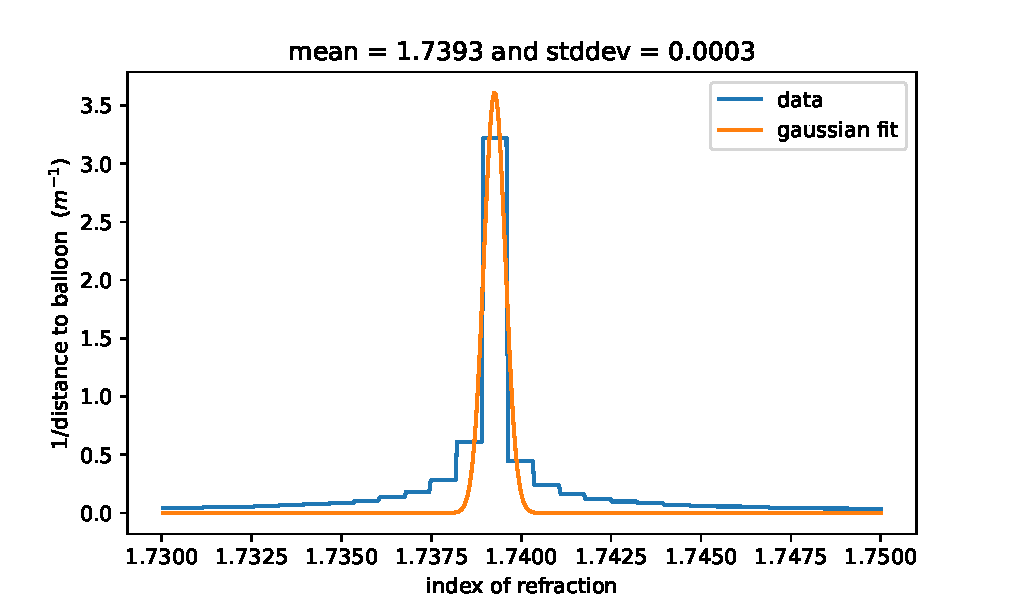
\includegraphics[width=0.8\textwidth]{GaussianFit.pdf}
	\caption{gaussian fit doesn't perfectly align with the data}
	\label{fig:GaussFit}
\end{figure}
\begin{figure}
	\centering
	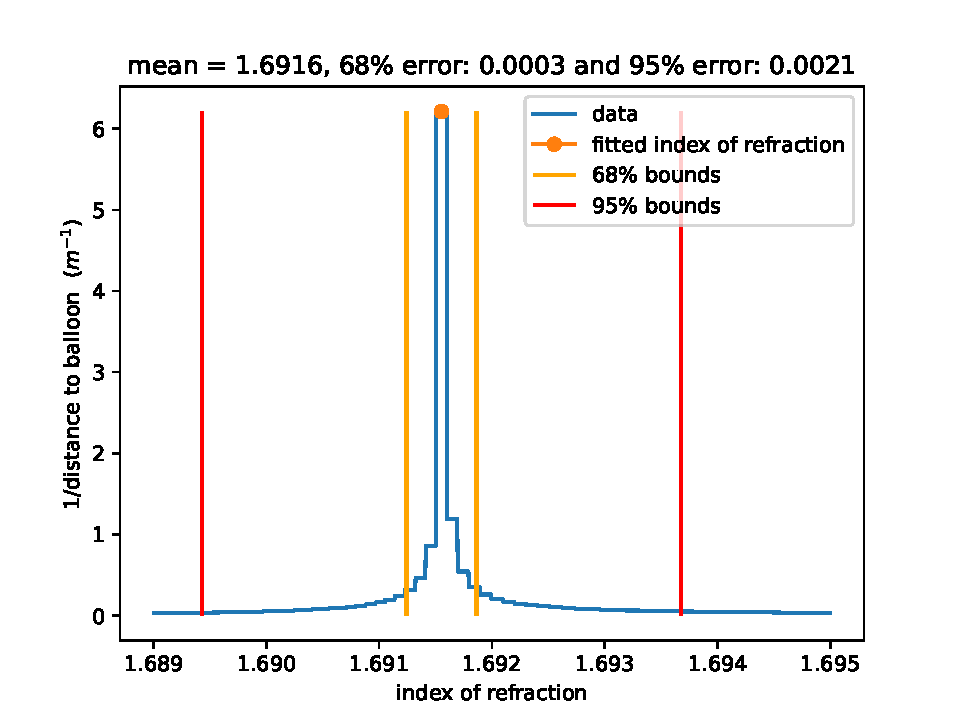
\includegraphics[width=0.8\textwidth]{Ch5And6Fit.pdf}
	\caption{Fit of channels 5 and 6}
	\label{fig:Ch5And6}
\end{figure}
\begin{figure}
	\centering
	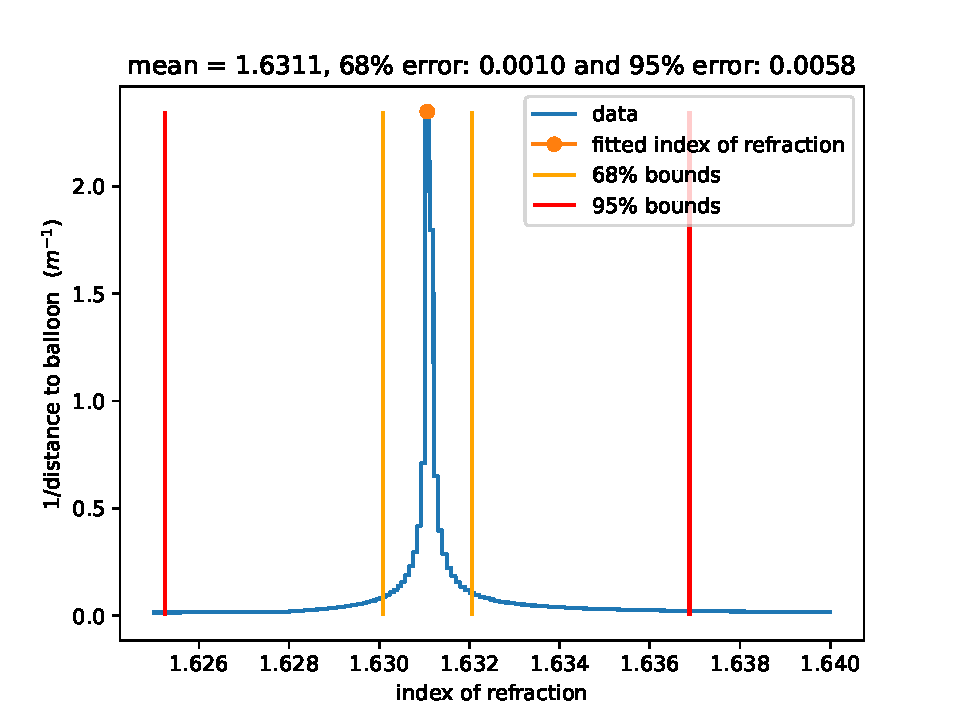
\includegraphics[width=0.8\textwidth]{Ch6And7Fit.pdf}
	\caption{Fit of channels 6 and 7}
	\label{fig:Ch6And7}
\end{figure}
\begin{figure}
	\centering
	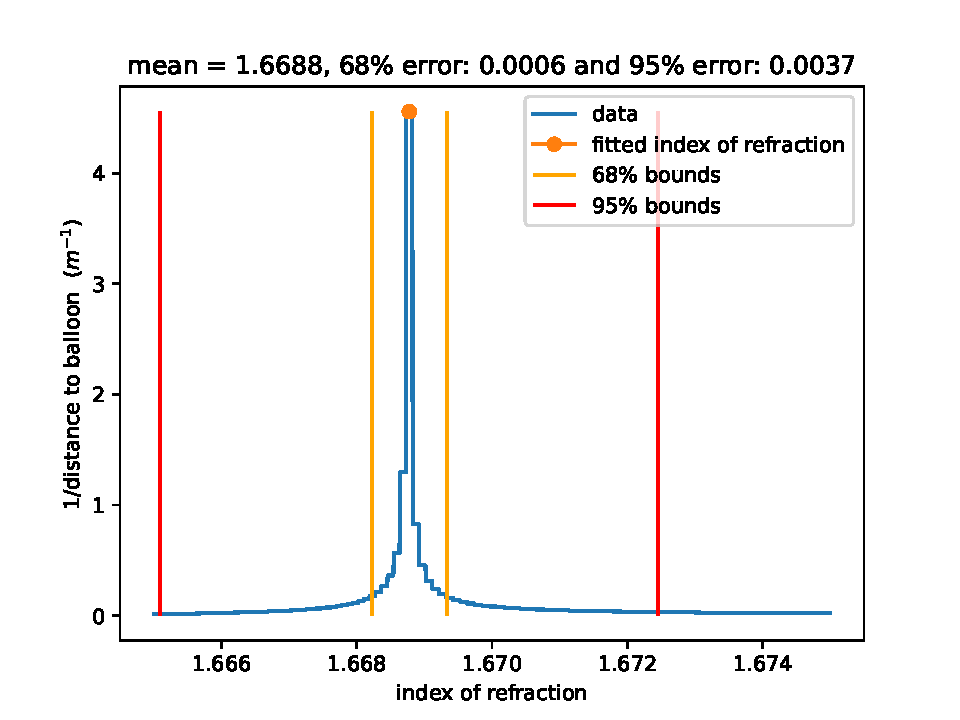
\includegraphics[width=0.8\textwidth]{Ch5And7Fit.pdf}
	\caption{Fit of channels 5 and 7}
	\label{fig:Ch5And7}
\end{figure}

\chapter{Balloon passbys under 5°\\ in the summer of 2022}
\label{app:5Deg}
\csvautotabular{tables/EventsBelow5DegPart1.csv}
\csvautotabular{tables/EventsBelow5DegPart2.csv}
\csvautotabular{tables/EventsBelow5DegPart3.csv}
\chapter{Balloon passbys under 10°\\ in the summer of 2022}
\label{app:10Deg}
\begin{table}[h!]
\csvautotabular{tables/EventsBelow10DegPart5.csv}
\end{table}
\begin{table}
\csvautotabular{tables/EventsBelow10DegPart1.csv}
\end{table}
\begin{table}
\csvautotabular{tables/EventsBelow10DegPart2.csv}
\end{table}
\begin{table}
\csvautotabular{tables/EventsBelow10DegPart3.csv}
\end{table}
\begin{table}
\csvautotabular{tables/EventsBelow10DegPart4.csv}
\end{table}


